% TeX encoding = utf8
% TeX spellcheck = pl_PL 
\documentclass[a4paper, 12pt]{article}
\usepackage[utf8]{inputenc}
\usepackage[polish]{babel}
\usepackage{polski}
\usepackage{graphicx}
\usepackage{listings}
\usepackage{amsfonts}
\usepackage{geometry}
\usepackage{subfigure}

\newgeometry{tmargin=1cm, bmargin=2cm, lmargin=1cm, rmargin=1cm}

\begin{document}
	\begin{center}
		
		\textbf{Sprawozdanie\\TST projekt 1\\Anna Wujek}
	\end{center}
	
	\paragraph{Skrypt (realizowany w octave)}
	\begin{itemize}
		\item Skrypt konstruuje macierz A wg wzoru $A = VDV^{-1}$, gdzie $V$ - podana macierz wektorów własnych, $D$ - macierz diagonalna z podanymi wartościami własnymi. Jeśli w widmie są wartości zespolone, należy podać je w formie $\sigma(A)=\{(a+bi),(a-bi)\}$ i zwracana jest macierz $[a,b;-b,a]$
		\item Wygenerowane punkty początkowe są rozmieszczone równomiernie na okręgu o zadanym promieniu.
		\item Trajektoria układu obliczana jest jako ciąg $x(t)=A^tx_0$, gdzie $x(0)=x_0$, $t = 0,1,2,3,...$ dla kolejnych podanych punktów początkowych $x_0$.
		\item Wektory własne obliczane są przy pomocy funkcji \verb|eig(A)|.
		\item Ilustrację trajektorii w przestrzeni stanów stanowi wykres ze zmiennymi stanu na osiach, pokazujący wzajemną zależność między nimi w czasie. Wykonywany dla różnych punktów początkowych, tworzy portret fazowy.
		\item Wykres $Az(\theta)$ rysowany jest na tle okręgu jednostkowego.
		\item Wektory $\lambda _iv_i,\quad \lambda _i \in \sigma (A)$ zostały przedstawione zarówno dla wektorów podanych przy tworzeniu macierzy, jak i dla wektorów obliczonych przez funkcję \verb|eig(A)|.
		\item Pole wektorowe rysowane jest dla siatki punktów początkowych (a nie dla okręgu) dla lepszej czytelności.
	\end{itemize}
	
	\paragraph{Interpretacja wartości własnych i wektorów własnych}
	\begin{itemize}
		
		\item \textbf{Wektory własne $v_i$}
		
		Z definicji: niezerowe wektory $x$ spełniające równanie $[\mathbb{I}_n\lambda-A]x = 0$, czyli $Ax=\lambda x$
		
		Są to wektory, które po przemnożeniu przez macierz A, pozostają tym samym wektorem (co najwyżej przeskalowanym przez parametr $\lambda$, czyli związaną z nim wartość własną). 
			
		Eksperymenty w skrypcie pokazały, że wektory własne podane przy tworzeniu macierzy oraz te obliczone przez funkcję \verb|eig(A)| leżą na tych samych prostych, a różnią się jedynie długością lub zwrotem. Wniosek: macierz może mieć wiele wektorów własnych związanych z daną wartością własną, lecz będą one leżeć na tych samych prostych.
		
		Wyjątek stanowi sytuacja, gdy obie wartości własne są identyczne (tj. $\lambda _1 = \lambda _2$). Wtedy macierz A znaleziona przy pomocy $A = VDV^{-1}$ ma postać $[\lambda, 0; 0, \lambda]$, a wektor własny jest dowolny.
		
		\begin{figure}[h]
			\begin{center}
				\subfigure[Wektory własne podane: (0.1,0.2 ; 3.2,-0.4)]{
					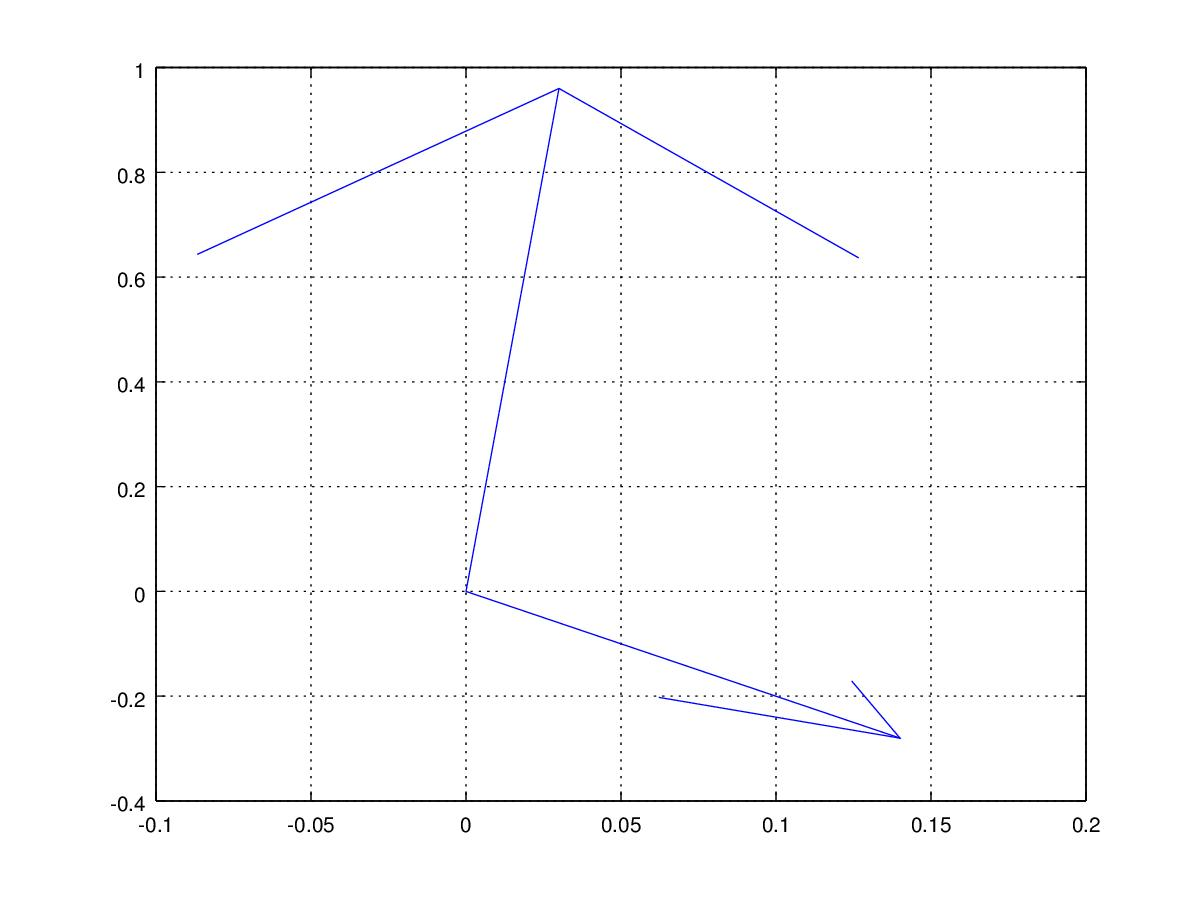
\includegraphics[width=0.3\linewidth]{img/wektory_wlasne_podane.jpg}}
				\subfigure[Wektory własne obliczone z eig(A): ( 0.447214,0.031235;-0.894427,0.999512)]{
					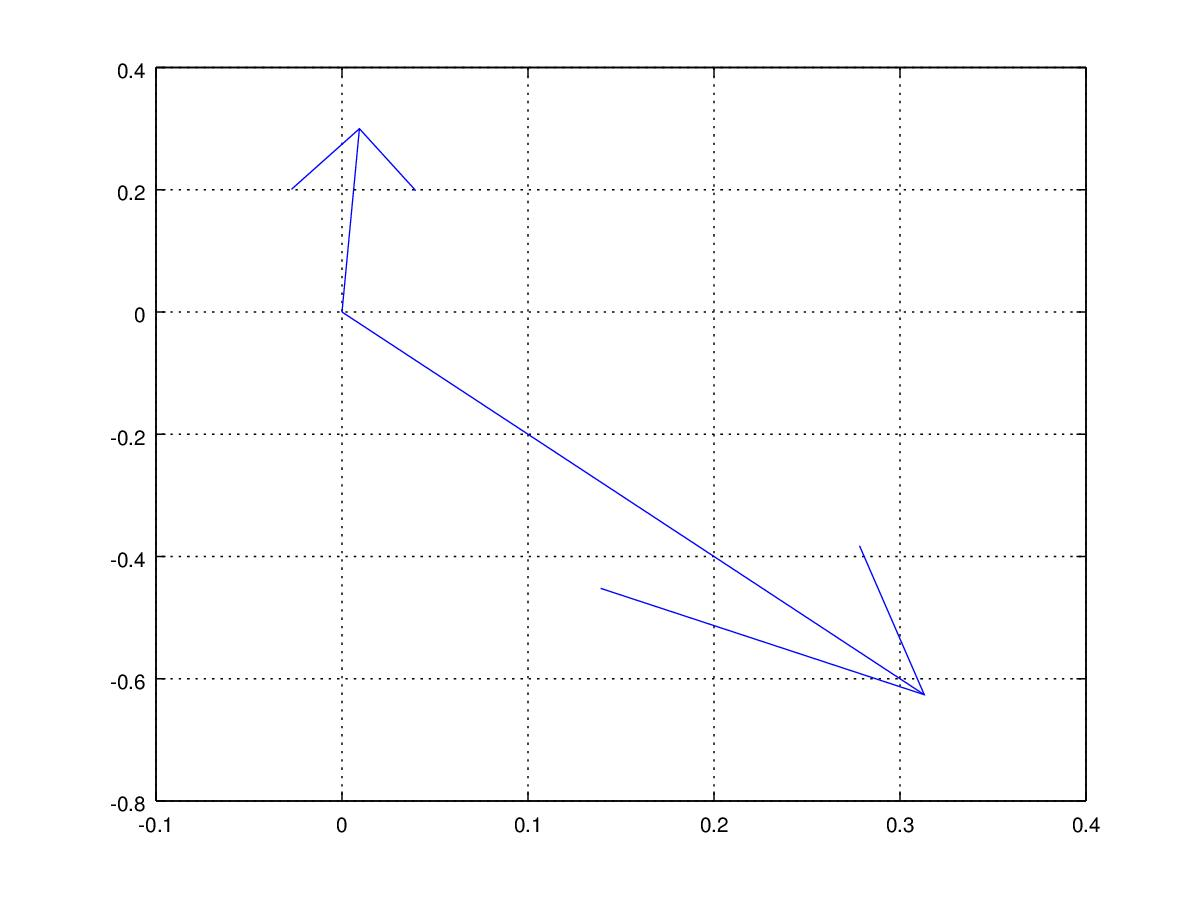
\includegraphics[width=0.3\linewidth]{img/wektory_wlasne_eig.jpg}}
				\caption{Ilustracja wektorów własnych}
			\end{center}
		\end{figure}
		
		\item \textbf{Wartości własne $\lambda _i$}
		
		Z definicji: rozwiązania wielomianu charakterystycznego macierzy A, czyli $det[\mathbb{I}_n\lambda-\mathbb{A}] = 0$.
		
		Związane z wektorami własnymi zgodnie z $Ax=\lambda x$.
		
		Wartości własne są biegunami układu opisanego macierzą A i wpływają na jego dynamikę. W zależności od wartości części rzeczywistej i urojonej zmieniają stabilność układu oraz kierunek zmian stanu w czasie. 
	\end{itemize}
	

	
	\paragraph{Zależność dynamiki od widma macierzy A}
	\begin{itemize}
		\item od wartości własnych zależy kształt dynamiki układu wokół punktów osobliwych, co jest dobrze widoczne na rysunku pola wektorowego. Dla podanego zadania jedynym punktem osobliwym jest $(0,0)$. Wektory pokazują kierunek zmian zmiennych stanu na płaszczyźnie fazowej.
		\begin{itemize}
			\item $\lambda _1, \lambda _2$ - rzeczywiste, mniejsze od 0 - węzeł stabilny
			\item $\lambda _1, \lambda _2$ - rzeczywiste, większe od 0 - węzeł niestabilny
			\item $\lambda _1, \lambda _2$ - rzeczywiste, jedna $>0$, druga $<0$ - siodło
			\item $\lambda _1, \lambda _2$ - zespolone sprzężone, z ujemną częścią rzeczywistą - ognisko stabilne
			\item $\lambda _1, \lambda _2$ - zespolone sprzężone, z dodatnią częścią rzeczywistą - ognisko niestabilne
			\item $\lambda _1, \lambda _2$ - zespolone sprzężone, z zerową częścią rzeczywistą - środek (oscylacje)
		\end{itemize}
		\begin{figure}[h]
			\begin{center}
				\subfigure[Węzeł stabilny]{
					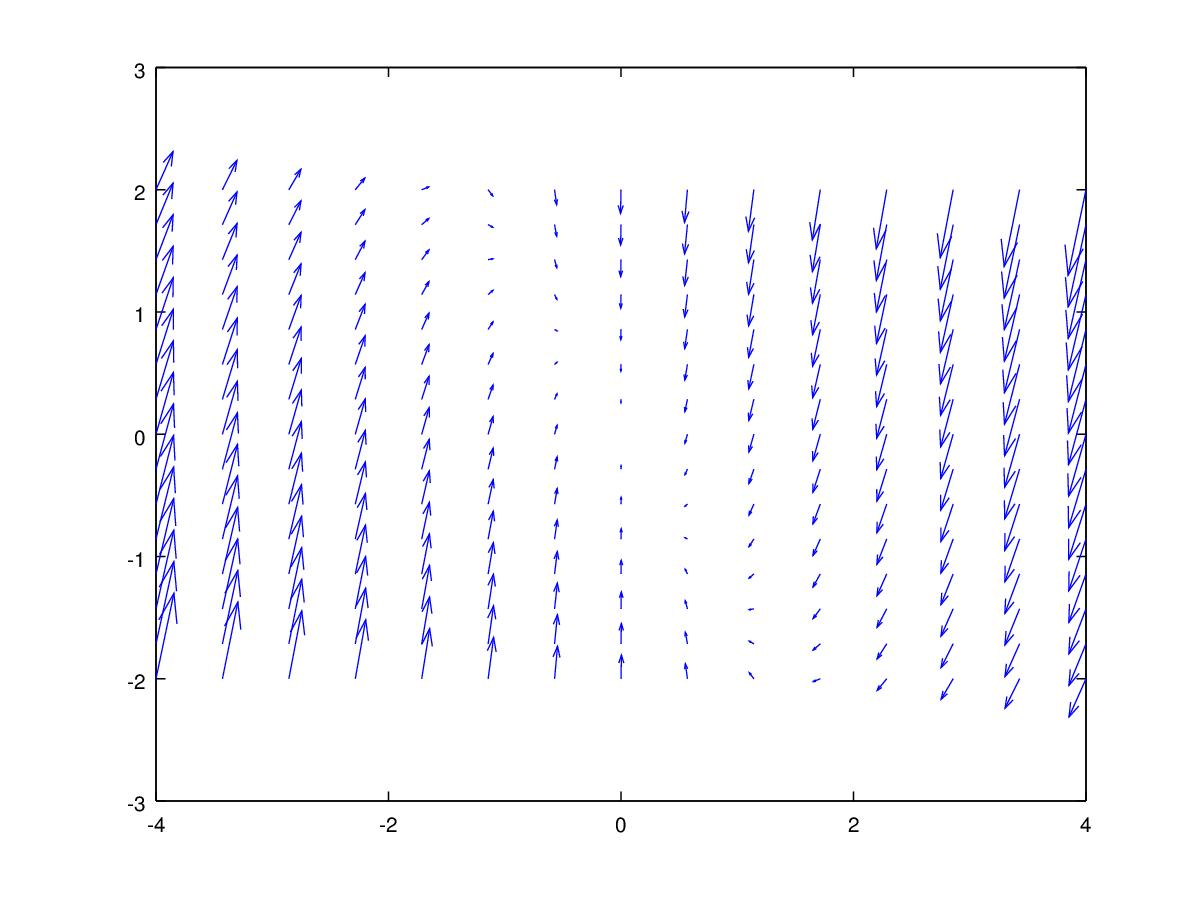
\includegraphics[width=0.3\linewidth]{img/wektory_wezel_stabilny.jpg}}
				\subfigure[Węzeł niestabilny]{
					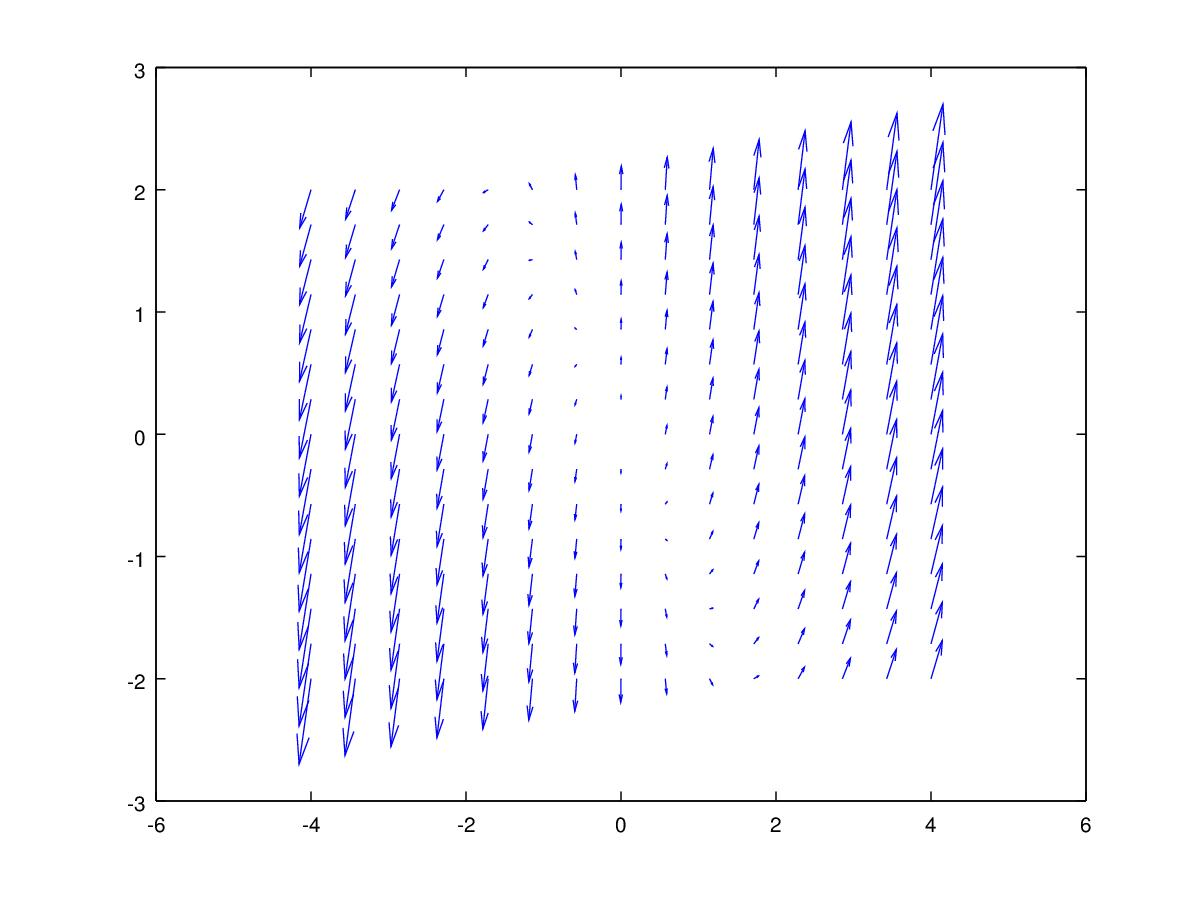
\includegraphics[width=0.3\linewidth]{img/wektory_wezel_niestabilny.jpg}}
				\subfigure[Siodło]{
					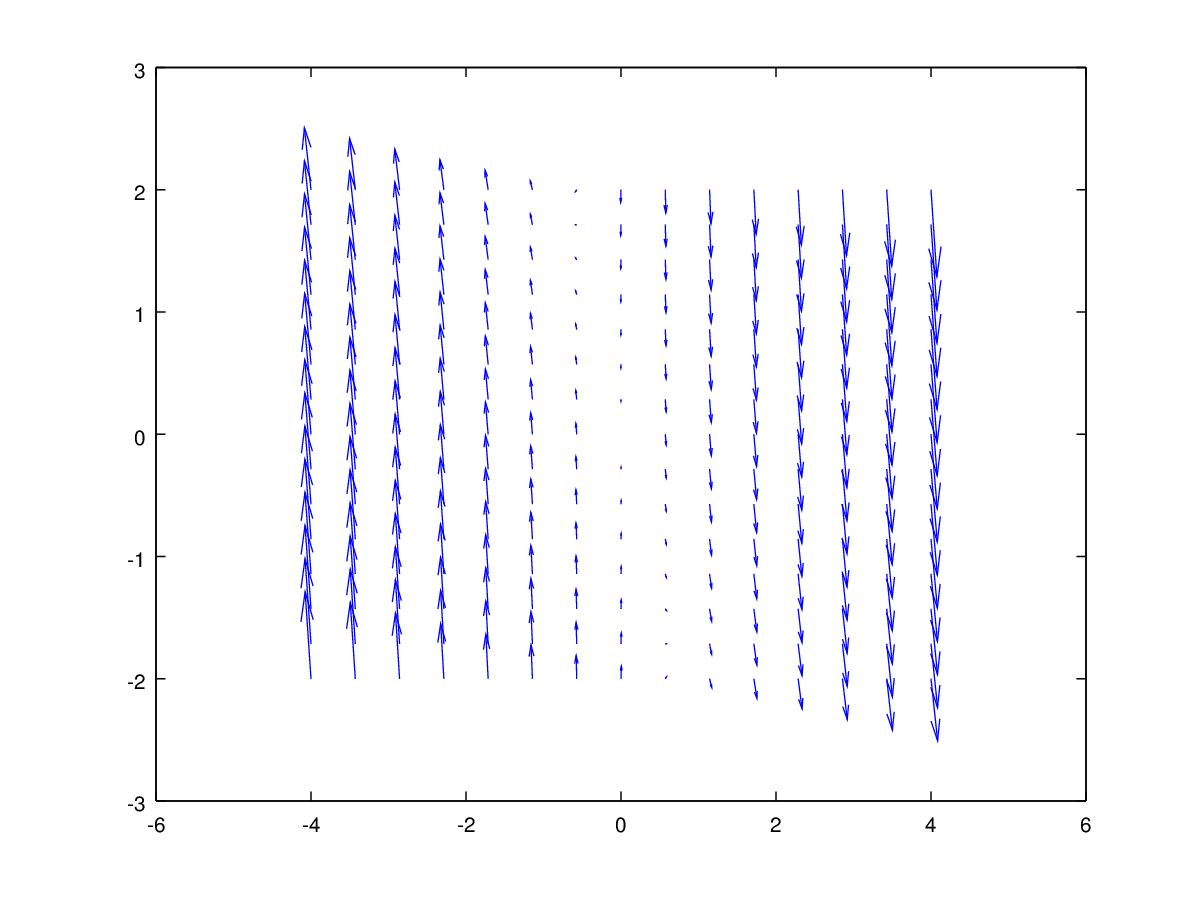
\includegraphics[width=0.3\linewidth]{img/wektory_siodlo.jpg}}
				\subfigure[Ognisko stabilne]{
					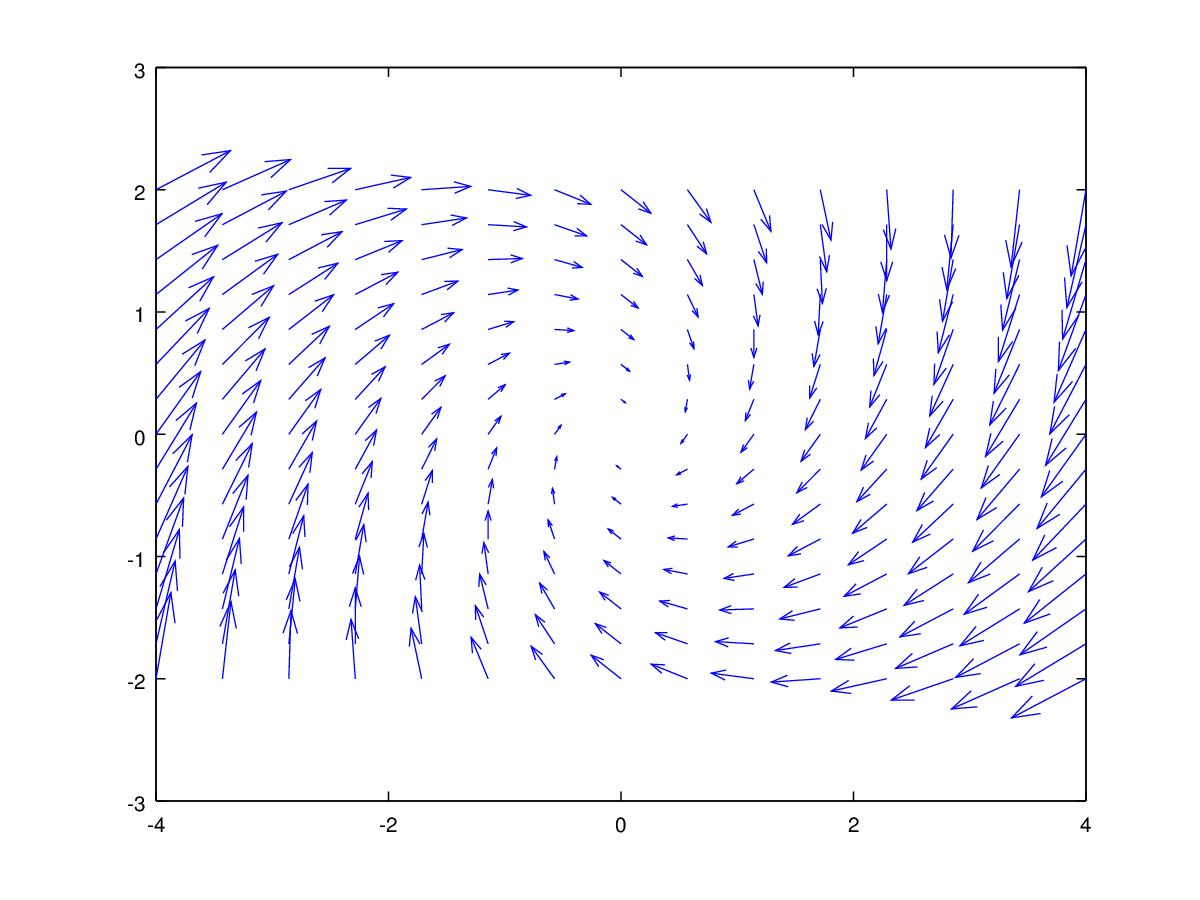
\includegraphics[width=0.3\linewidth]{img/wektory_ognisko_stabilne.jpg}}
				\subfigure[Ognisko niestabilne]{
					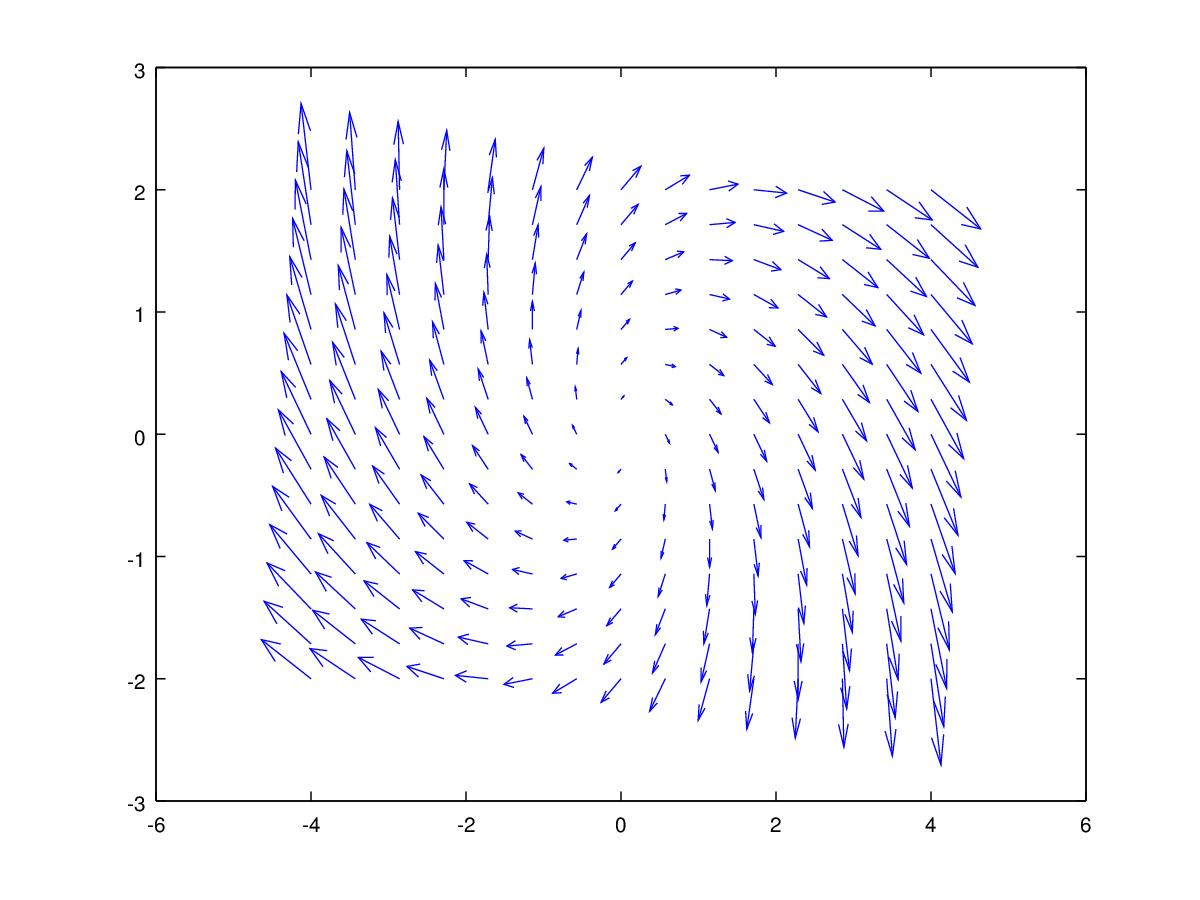
\includegraphics[width=0.3\linewidth]{img/wektory_ognisko_niestabilne.jpg}}
				\subfigure[Środek]{
					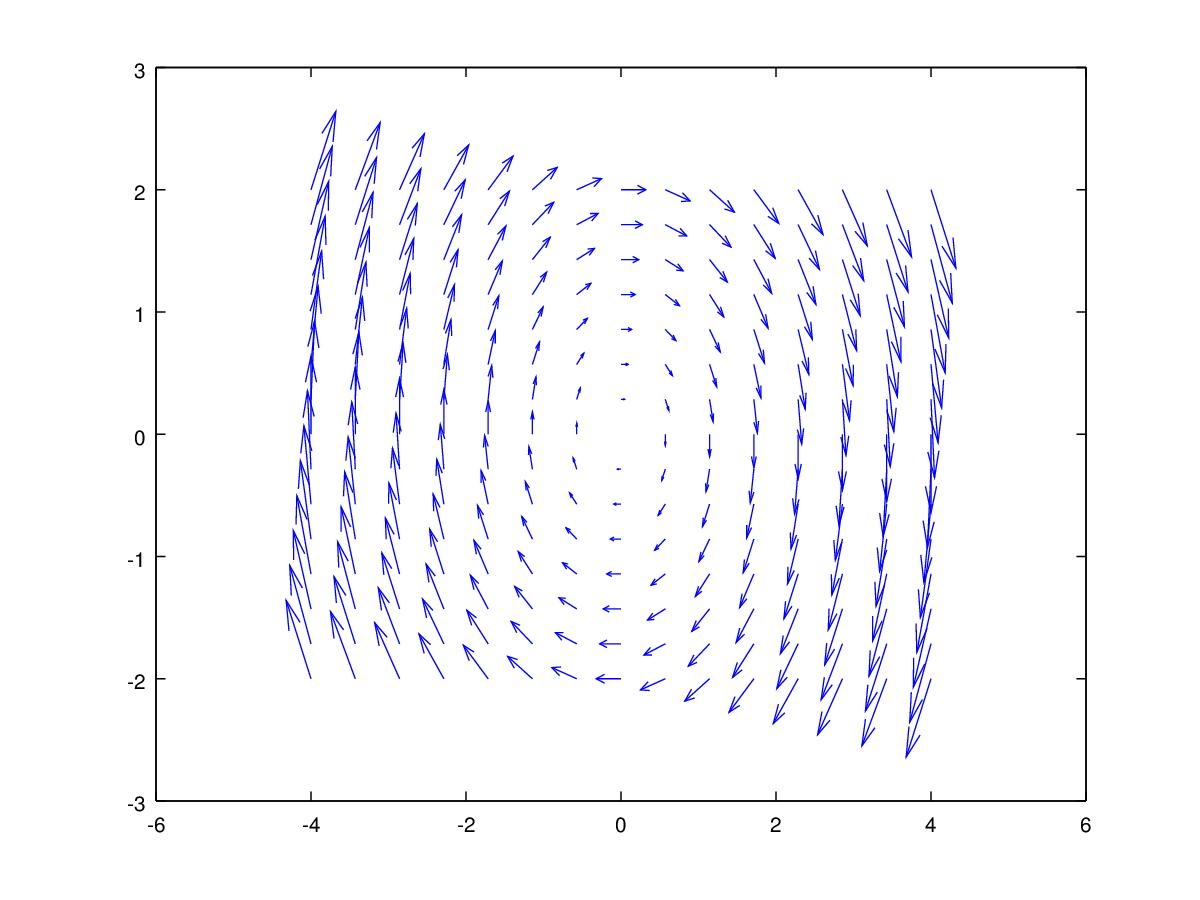
\includegraphics[width=0.3\linewidth]{img/wektory_srodek.jpg}}
				\caption{Pola wektorowe}
			\end{center}
		\end{figure}
		\item Stabilność układu
		\begin{itemize}
			\item Aby układ był stabilny, wszystkie wartości własne muszą leżeć na płaszczyźnie zespolonej w kole jednostkowym, bo wtedy $\lim\limits_{t\rightarrow \infty}A^t = 0$.
			\item Jeśli chociaż jedna ma moduł $>1$, układ staje się niestabilny, bo wtedy $\lim\limits_{t\rightarrow\infty}A^t = \pm\infty$.
			\item Jeśli obie wartości własne mają moduły $=1$, układ oscyluje wokół punktu $(0,0)$ i nie zbiega do żadnej wartości.
			\item Jeśli jedna z wartości ma moduł $<1$, a druga $=1$, układ nie zbiega do 0 ani nie rozbiega się do nieskończoności ani nie oscyluje cały czas, tylko w zależności od punktu początkowego zbiega do różnych wartości.
		\end{itemize}  
		\begin{figure}[h]
			\begin{center}
				\subfigure[$|\lambda _1|,|\lambda _2| < 1$ - stabilny]{
					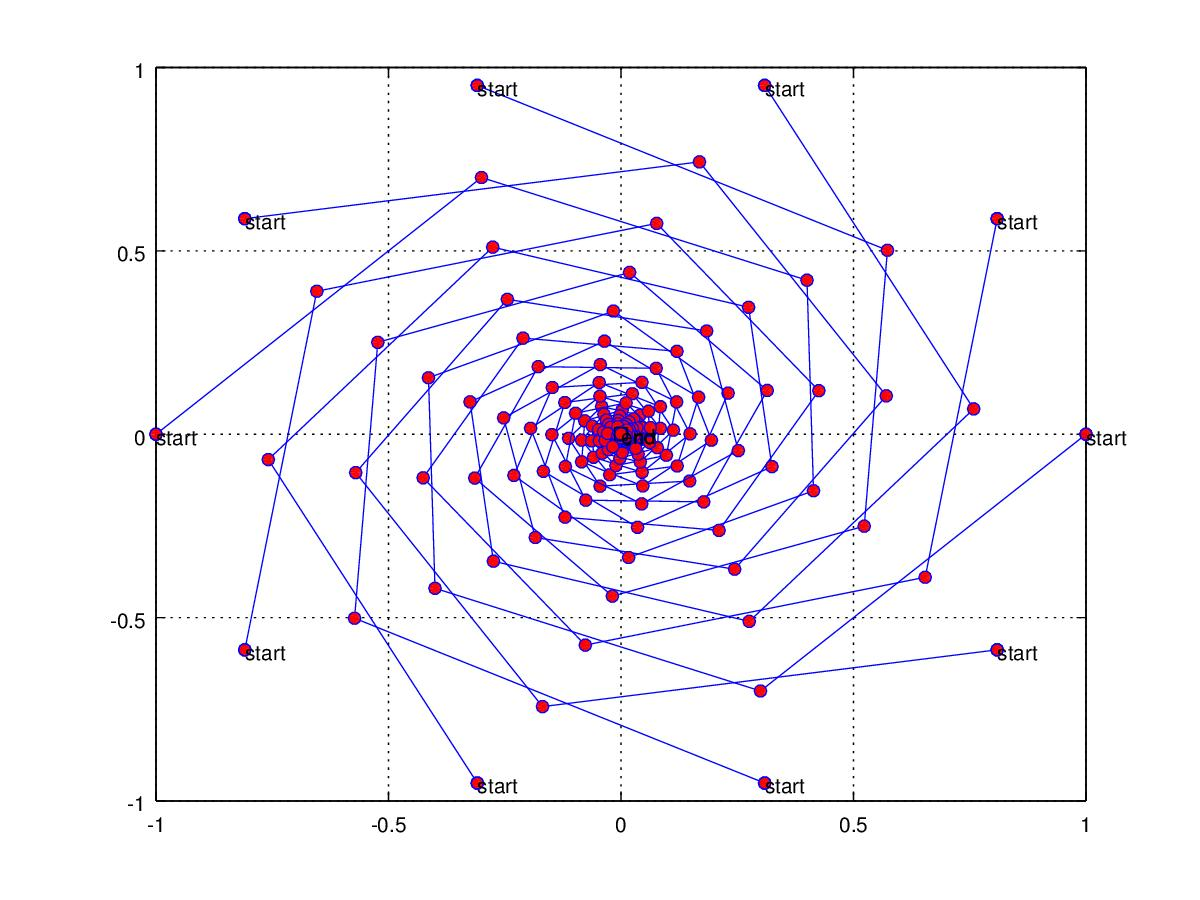
\includegraphics[width=0.4\linewidth]{img/portret_stabilny.jpg}}
				\subfigure[$|\lambda _1| > 1$ - niestabilny]{
					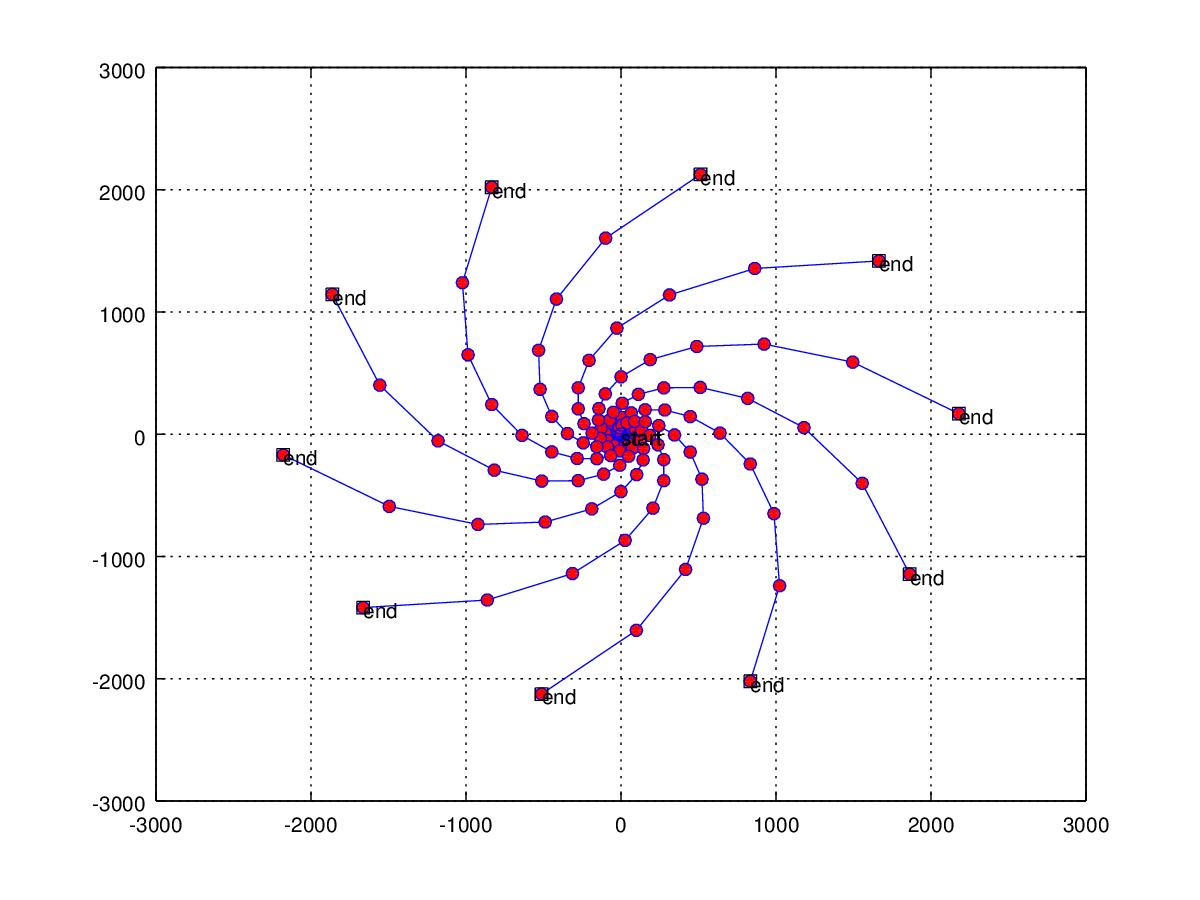
\includegraphics[width=0.4\linewidth]{img/portret_niestabilny.jpg}}
				\subfigure[$|\lambda _1|,|\lambda _2| = 1$ - oscylacje]{
					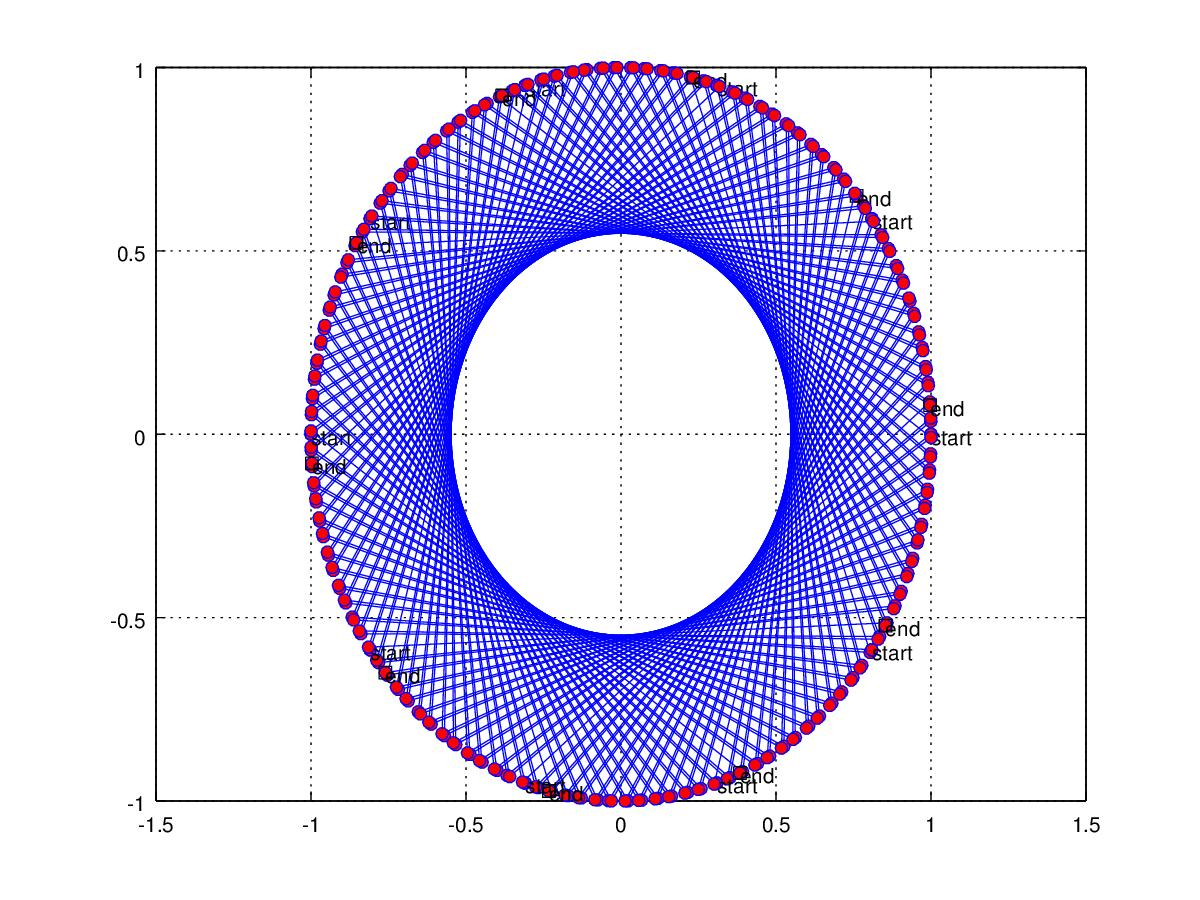
\includegraphics[width=0.4\linewidth]{img/portret_oscylacje.jpg}}
				\subfigure[$|\lambda _1| = 1, |\lambda _2|<1$ - zbiega do różnych punktów w zależności od punktu początkowego]{
					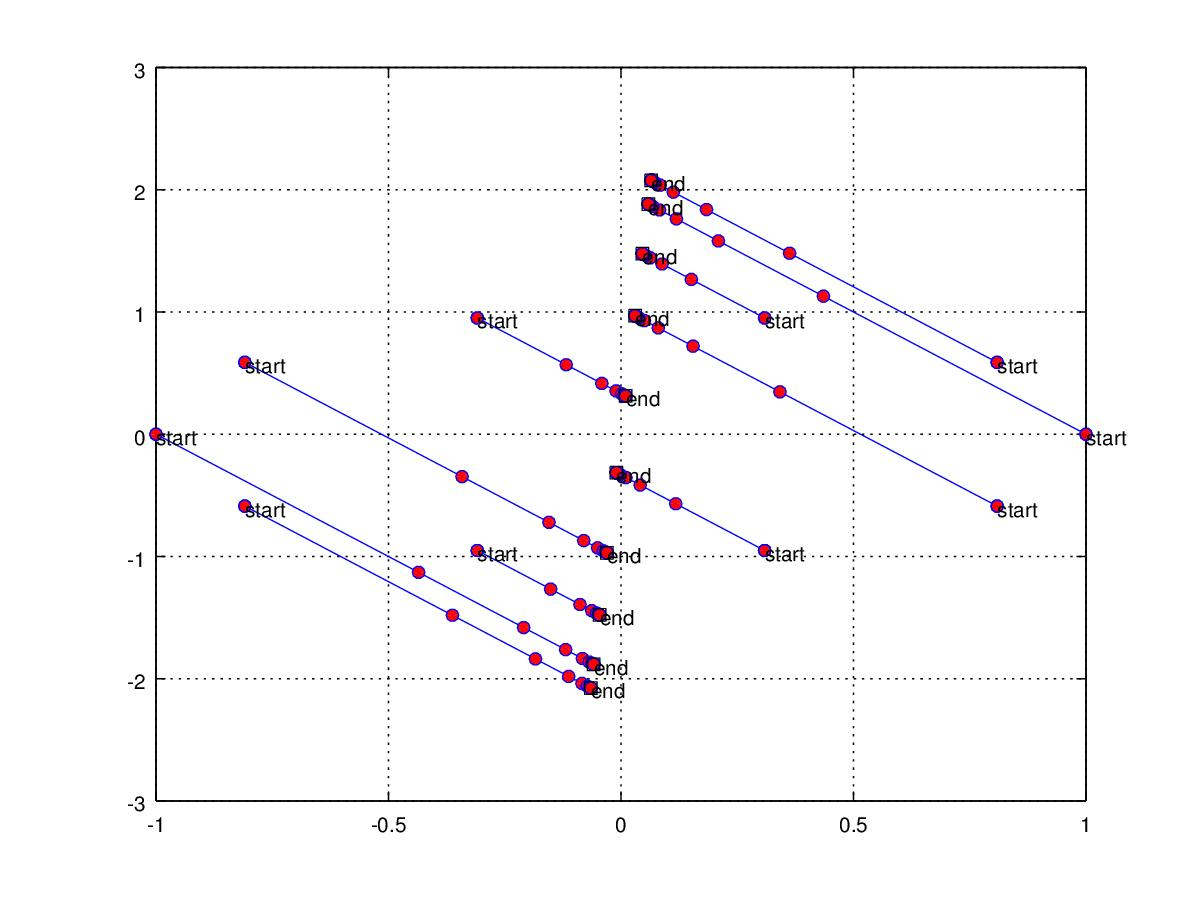
\includegraphics[width=0.4\linewidth]{img/portret_pol_oscylacje.jpg}}
				\caption{Portrety fazowe dla różnych $\lambda$}
			\end{center}
		\end{figure} 
	\end{itemize}
	
	
	
	
\end{document}



